\documentclass[11pt]{article}
% =======================================================================
%   Shared style for CS 300 notes.
%   Usage: place `% =======================================================================
%   Shared style for CS 300 notes.
%   Usage: place `% =======================================================================
%   Shared style for CS 300 notes.
%   Usage: place `\input{../../notes-style.tex}` right after \documentclass
%   in each chapter's lectures.tex and notes.tex.
% =======================================================================

% ---- Layout -----------------------------------------------------------
\usepackage[margin=1in]{geometry}
\usepackage{parskip}        % space between paragraphs, no indent
\usepackage{microtype}      % subtle kerning/spacing improvements

% ---- Colors (muted palette, easy on light-sensitive eyes) -------------
\usepackage{xcolor}
\definecolor{pagebg}       {HTML}{FAF6F0}  % warm cream background
\definecolor{bodyfg}       {HTML}{3D3A36}  % warm dark gray body text
\definecolor{heading}      {HTML}{3D6A6B}  % muted teal
\definecolor{subheading}   {HTML}{5B7A9C}  % dusty blue
\definecolor{accent}       {HTML}{8A6B4A}  % warm tan
\definecolor{linkcol}      {HTML}{5B7A9C}  % same as subheading
\definecolor{mutedtext}    {HTML}{6B6560}  % secondary / caption text
\definecolor{rulecol}      {HTML}{C8BFB0}  % separator / rule

% Callout box palette
\definecolor{defnFrame}    {HTML}{9DB89B}  \definecolor{defnBack}    {HTML}{EEF2E8}
\definecolor{ideaFrame}    {HTML}{9FB4CD}  \definecolor{ideaBack}    {HTML}{E8EEF5}
\definecolor{warnFrame}    {HTML}{CFAE87}  \definecolor{warnBack}    {HTML}{F5EDDF}
\definecolor{noteFrame}    {HTML}{BFA6AE}  \definecolor{noteBack}    {HTML}{F2E8EE}
\definecolor{exFrame}      {HTML}{9FBDBD}  \definecolor{exBack}      {HTML}{E8F0F0}
\definecolor{codeBack}     {HTML}{F3EDE2}
\definecolor{codeBorder}   {HTML}{D4CBBA}
\definecolor{codeKeyword}  {HTML}{6B4F7A}
\definecolor{codeString}   {HTML}{8A6B4A}
\definecolor{codeComment}  {HTML}{8A857F}

% ---- Page background + base text color --------------------------------
\usepackage{pagecolor}
\pagecolor{pagebg}
\color{bodyfg}

% ---- Fonts ------------------------------------------------------------
\usepackage[T1]{fontenc}
\IfFileExists{libertine.sty}{%
    \usepackage{libertine}      % warm, readable serif
    \usepackage[scaled=0.95]{inconsolata}  % softer monospace
}{}

% ---- Hyperref ---------------------------------------------------------
\usepackage{hyperref}
\hypersetup{
    colorlinks=true,
    linkcolor=linkcol,
    urlcolor=linkcol,
    citecolor=linkcol,
    pdfborder={0 0 0},
}

% ---- Section styling --------------------------------------------------
\usepackage[explicit]{titlesec}
\titleformat{\section}
    {\color{heading}\Large\bfseries}
    {\color{heading}\thesection\hspace{0.6em}}{0pt}{#1}
\titleformat{\subsection}
    {\color{subheading}\large\bfseries}
    {\color{subheading}\thesubsection\hspace{0.5em}}{0pt}{#1}
\titleformat{\subsubsection}
    {\color{accent}\normalsize\bfseries}
    {\color{accent}\thesubsubsection\hspace{0.5em}}{0pt}{#1}
\titleformat{\paragraph}[runin]
    {\color{accent}\bfseries}{}{0pt}{#1.}

\titlespacing*{\section}{0pt}{1.6em}{0.6em}
\titlespacing*{\subsection}{0pt}{1.2em}{0.4em}

% ---- Enumerate / itemize spacing --------------------------------------
\usepackage{enumitem}
\setlist[itemize]{leftmargin=1.4em, itemsep=2pt, topsep=4pt}
\setlist[enumerate]{leftmargin=1.6em, itemsep=2pt, topsep=4pt}

% ---- Code listings ----------------------------------------------------
\usepackage{listings}
\lstdefinestyle{notescode}{
    backgroundcolor=\color{codeBack},
    basicstyle=\ttfamily\small\color{bodyfg},
    keywordstyle=\color{codeKeyword}\bfseries,
    stringstyle=\color{codeString},
    commentstyle=\color{codeComment}\itshape,
    frame=single,
    framesep=6pt,
    rulecolor=\color{codeBorder},
    showstringspaces=false,
    breaklines=true,
    xleftmargin=10pt,
    xrightmargin=10pt,
    aboveskip=8pt,
    belowskip=8pt,
}
\lstset{style=notescode}

% ---- Callout boxes (tcolorbox) ----------------------------------------
\usepackage[most]{tcolorbox}

\newtcolorbox{defnbox}[1][]{
    enhanced, breakable,
    colback=defnBack, colframe=defnFrame, coltitle=bodyfg,
    title={\bfseries Definition \textemdash\ #1},
    fonttitle=\bfseries,
    boxrule=0.5pt, arc=2pt, left=8pt, right=8pt, top=6pt, bottom=6pt,
    attach boxed title to top left={xshift=10pt, yshift=-6pt},
    boxed title style={colback=defnFrame, colframe=defnFrame, arc=2pt},
    before skip=8pt, after skip=8pt,
}
\newtcolorbox{ideabox}[1][]{
    enhanced, breakable,
    colback=ideaBack, colframe=ideaFrame, coltitle=bodyfg,
    title={\bfseries Key idea #1},
    boxrule=0.5pt, arc=2pt, left=8pt, right=8pt, top=6pt, bottom=6pt,
    attach boxed title to top left={xshift=10pt, yshift=-6pt},
    boxed title style={colback=ideaFrame, colframe=ideaFrame, arc=2pt},
    before skip=8pt, after skip=8pt,
}
\newtcolorbox{warnbox}[1][]{
    enhanced, breakable,
    colback=warnBack, colframe=warnFrame, coltitle=bodyfg,
    title={\bfseries Gotcha #1},
    boxrule=0.5pt, arc=2pt, left=8pt, right=8pt, top=6pt, bottom=6pt,
    attach boxed title to top left={xshift=10pt, yshift=-6pt},
    boxed title style={colback=warnFrame, colframe=warnFrame, arc=2pt},
    before skip=8pt, after skip=8pt,
}
\newtcolorbox{notebox}[1][]{
    enhanced, breakable,
    colback=noteBack, colframe=noteFrame, coltitle=bodyfg,
    title={\bfseries Aside #1},
    boxrule=0.5pt, arc=2pt, left=8pt, right=8pt, top=6pt, bottom=6pt,
    attach boxed title to top left={xshift=10pt, yshift=-6pt},
    boxed title style={colback=noteFrame, colframe=noteFrame, arc=2pt},
    before skip=8pt, after skip=8pt,
}
\newtcolorbox{examplebox}[1][]{
    enhanced, breakable,
    colback=exBack, colframe=exFrame, coltitle=bodyfg,
    title={\bfseries Example #1},
    boxrule=0.5pt, arc=2pt, left=8pt, right=8pt, top=6pt, bottom=6pt,
    attach boxed title to top left={xshift=10pt, yshift=-6pt},
    boxed title style={colback=exFrame, colframe=exFrame, arc=2pt},
    before skip=8pt, after skip=8pt,
}

% ---- TikZ graph styles (added 2026-04-25 for ch_10 augmentation) ------
% tcolorbox[most] already loads tikz; this block declares the libraries
% + shared `vertex` / `edge` styles used by ch_10's general directed-graph
% diagrams. ch_9's tree-style TikZ uses inline overrides and is
% unaffected. Simple circle nodes + arrow edges only -- no production
% styling.
\usetikzlibrary{arrows.meta, positioning, calc}
\tikzset{
    vertex/.style={circle, draw, minimum size=7mm, inner sep=0pt,
                   font=\small, thick},
    vsource/.style={vertex, fill=ideaBack},
    vdone/.style={vertex, fill=defnBack},
    edge/.style={->, >=Stealth, thick},
    uedge/.style={-, thick},
    treeedge/.style={->, >=Stealth, thick},
    backedge/.style={->, >=Stealth, thick, dashed, red!70!black},
    fwdedge/.style={->, >=Stealth, thick, blue!60!black},
    crossedge/.style={->, >=Stealth, thick, green!50!black, dotted},
    mstedge/.style={-, very thick, accent},
}

% ---- Title block ------------------------------------------------------
\usepackage{titling}
\pretitle{\begin{center}\color{heading}\LARGE\bfseries}
\posttitle{\end{center}\vskip -0.4em}
\preauthor{\begin{center}\color{mutedtext}\normalsize}
\postauthor{\end{center}}
\predate{\begin{center}\color{mutedtext}\small}
\postdate{\end{center}\vspace{0.4em}{\color{rulecol}\hrule height 0.4pt}\vspace{1.2em}}
` right after \documentclass
%   in each chapter's lectures.tex and notes.tex.
% =======================================================================

% ---- Layout -----------------------------------------------------------
\usepackage[margin=1in]{geometry}
\usepackage{parskip}        % space between paragraphs, no indent
\usepackage{microtype}      % subtle kerning/spacing improvements

% ---- Colors (muted palette, easy on light-sensitive eyes) -------------
\usepackage{xcolor}
\definecolor{pagebg}       {HTML}{FAF6F0}  % warm cream background
\definecolor{bodyfg}       {HTML}{3D3A36}  % warm dark gray body text
\definecolor{heading}      {HTML}{3D6A6B}  % muted teal
\definecolor{subheading}   {HTML}{5B7A9C}  % dusty blue
\definecolor{accent}       {HTML}{8A6B4A}  % warm tan
\definecolor{linkcol}      {HTML}{5B7A9C}  % same as subheading
\definecolor{mutedtext}    {HTML}{6B6560}  % secondary / caption text
\definecolor{rulecol}      {HTML}{C8BFB0}  % separator / rule

% Callout box palette
\definecolor{defnFrame}    {HTML}{9DB89B}  \definecolor{defnBack}    {HTML}{EEF2E8}
\definecolor{ideaFrame}    {HTML}{9FB4CD}  \definecolor{ideaBack}    {HTML}{E8EEF5}
\definecolor{warnFrame}    {HTML}{CFAE87}  \definecolor{warnBack}    {HTML}{F5EDDF}
\definecolor{noteFrame}    {HTML}{BFA6AE}  \definecolor{noteBack}    {HTML}{F2E8EE}
\definecolor{exFrame}      {HTML}{9FBDBD}  \definecolor{exBack}      {HTML}{E8F0F0}
\definecolor{codeBack}     {HTML}{F3EDE2}
\definecolor{codeBorder}   {HTML}{D4CBBA}
\definecolor{codeKeyword}  {HTML}{6B4F7A}
\definecolor{codeString}   {HTML}{8A6B4A}
\definecolor{codeComment}  {HTML}{8A857F}

% ---- Page background + base text color --------------------------------
\usepackage{pagecolor}
\pagecolor{pagebg}
\color{bodyfg}

% ---- Fonts ------------------------------------------------------------
\usepackage[T1]{fontenc}
\IfFileExists{libertine.sty}{%
    \usepackage{libertine}      % warm, readable serif
    \usepackage[scaled=0.95]{inconsolata}  % softer monospace
}{}

% ---- Hyperref ---------------------------------------------------------
\usepackage{hyperref}
\hypersetup{
    colorlinks=true,
    linkcolor=linkcol,
    urlcolor=linkcol,
    citecolor=linkcol,
    pdfborder={0 0 0},
}

% ---- Section styling --------------------------------------------------
\usepackage[explicit]{titlesec}
\titleformat{\section}
    {\color{heading}\Large\bfseries}
    {\color{heading}\thesection\hspace{0.6em}}{0pt}{#1}
\titleformat{\subsection}
    {\color{subheading}\large\bfseries}
    {\color{subheading}\thesubsection\hspace{0.5em}}{0pt}{#1}
\titleformat{\subsubsection}
    {\color{accent}\normalsize\bfseries}
    {\color{accent}\thesubsubsection\hspace{0.5em}}{0pt}{#1}
\titleformat{\paragraph}[runin]
    {\color{accent}\bfseries}{}{0pt}{#1.}

\titlespacing*{\section}{0pt}{1.6em}{0.6em}
\titlespacing*{\subsection}{0pt}{1.2em}{0.4em}

% ---- Enumerate / itemize spacing --------------------------------------
\usepackage{enumitem}
\setlist[itemize]{leftmargin=1.4em, itemsep=2pt, topsep=4pt}
\setlist[enumerate]{leftmargin=1.6em, itemsep=2pt, topsep=4pt}

% ---- Code listings ----------------------------------------------------
\usepackage{listings}
\lstdefinestyle{notescode}{
    backgroundcolor=\color{codeBack},
    basicstyle=\ttfamily\small\color{bodyfg},
    keywordstyle=\color{codeKeyword}\bfseries,
    stringstyle=\color{codeString},
    commentstyle=\color{codeComment}\itshape,
    frame=single,
    framesep=6pt,
    rulecolor=\color{codeBorder},
    showstringspaces=false,
    breaklines=true,
    xleftmargin=10pt,
    xrightmargin=10pt,
    aboveskip=8pt,
    belowskip=8pt,
}
\lstset{style=notescode}

% ---- Callout boxes (tcolorbox) ----------------------------------------
\usepackage[most]{tcolorbox}

\newtcolorbox{defnbox}[1][]{
    enhanced, breakable,
    colback=defnBack, colframe=defnFrame, coltitle=bodyfg,
    title={\bfseries Definition \textemdash\ #1},
    fonttitle=\bfseries,
    boxrule=0.5pt, arc=2pt, left=8pt, right=8pt, top=6pt, bottom=6pt,
    attach boxed title to top left={xshift=10pt, yshift=-6pt},
    boxed title style={colback=defnFrame, colframe=defnFrame, arc=2pt},
    before skip=8pt, after skip=8pt,
}
\newtcolorbox{ideabox}[1][]{
    enhanced, breakable,
    colback=ideaBack, colframe=ideaFrame, coltitle=bodyfg,
    title={\bfseries Key idea #1},
    boxrule=0.5pt, arc=2pt, left=8pt, right=8pt, top=6pt, bottom=6pt,
    attach boxed title to top left={xshift=10pt, yshift=-6pt},
    boxed title style={colback=ideaFrame, colframe=ideaFrame, arc=2pt},
    before skip=8pt, after skip=8pt,
}
\newtcolorbox{warnbox}[1][]{
    enhanced, breakable,
    colback=warnBack, colframe=warnFrame, coltitle=bodyfg,
    title={\bfseries Gotcha #1},
    boxrule=0.5pt, arc=2pt, left=8pt, right=8pt, top=6pt, bottom=6pt,
    attach boxed title to top left={xshift=10pt, yshift=-6pt},
    boxed title style={colback=warnFrame, colframe=warnFrame, arc=2pt},
    before skip=8pt, after skip=8pt,
}
\newtcolorbox{notebox}[1][]{
    enhanced, breakable,
    colback=noteBack, colframe=noteFrame, coltitle=bodyfg,
    title={\bfseries Aside #1},
    boxrule=0.5pt, arc=2pt, left=8pt, right=8pt, top=6pt, bottom=6pt,
    attach boxed title to top left={xshift=10pt, yshift=-6pt},
    boxed title style={colback=noteFrame, colframe=noteFrame, arc=2pt},
    before skip=8pt, after skip=8pt,
}
\newtcolorbox{examplebox}[1][]{
    enhanced, breakable,
    colback=exBack, colframe=exFrame, coltitle=bodyfg,
    title={\bfseries Example #1},
    boxrule=0.5pt, arc=2pt, left=8pt, right=8pt, top=6pt, bottom=6pt,
    attach boxed title to top left={xshift=10pt, yshift=-6pt},
    boxed title style={colback=exFrame, colframe=exFrame, arc=2pt},
    before skip=8pt, after skip=8pt,
}

% ---- TikZ graph styles (added 2026-04-25 for ch_10 augmentation) ------
% tcolorbox[most] already loads tikz; this block declares the libraries
% + shared `vertex` / `edge` styles used by ch_10's general directed-graph
% diagrams. ch_9's tree-style TikZ uses inline overrides and is
% unaffected. Simple circle nodes + arrow edges only -- no production
% styling.
\usetikzlibrary{arrows.meta, positioning, calc}
\tikzset{
    vertex/.style={circle, draw, minimum size=7mm, inner sep=0pt,
                   font=\small, thick},
    vsource/.style={vertex, fill=ideaBack},
    vdone/.style={vertex, fill=defnBack},
    edge/.style={->, >=Stealth, thick},
    uedge/.style={-, thick},
    treeedge/.style={->, >=Stealth, thick},
    backedge/.style={->, >=Stealth, thick, dashed, red!70!black},
    fwdedge/.style={->, >=Stealth, thick, blue!60!black},
    crossedge/.style={->, >=Stealth, thick, green!50!black, dotted},
    mstedge/.style={-, very thick, accent},
}

% ---- Title block ------------------------------------------------------
\usepackage{titling}
\pretitle{\begin{center}\color{heading}\LARGE\bfseries}
\posttitle{\end{center}\vskip -0.4em}
\preauthor{\begin{center}\color{mutedtext}\normalsize}
\postauthor{\end{center}}
\predate{\begin{center}\color{mutedtext}\small}
\postdate{\end{center}\vspace{0.4em}{\color{rulecol}\hrule height 0.4pt}\vspace{1.2em}}
` right after \documentclass
%   in each chapter's lectures.tex and notes.tex.
% =======================================================================

% ---- Layout -----------------------------------------------------------
\usepackage[margin=1in]{geometry}
\usepackage{parskip}        % space between paragraphs, no indent
\usepackage{microtype}      % subtle kerning/spacing improvements

% ---- Colors (muted palette, easy on light-sensitive eyes) -------------
\usepackage{xcolor}
\definecolor{pagebg}       {HTML}{FAF6F0}  % warm cream background
\definecolor{bodyfg}       {HTML}{3D3A36}  % warm dark gray body text
\definecolor{heading}      {HTML}{3D6A6B}  % muted teal
\definecolor{subheading}   {HTML}{5B7A9C}  % dusty blue
\definecolor{accent}       {HTML}{8A6B4A}  % warm tan
\definecolor{linkcol}      {HTML}{5B7A9C}  % same as subheading
\definecolor{mutedtext}    {HTML}{6B6560}  % secondary / caption text
\definecolor{rulecol}      {HTML}{C8BFB0}  % separator / rule

% Callout box palette
\definecolor{defnFrame}    {HTML}{9DB89B}  \definecolor{defnBack}    {HTML}{EEF2E8}
\definecolor{ideaFrame}    {HTML}{9FB4CD}  \definecolor{ideaBack}    {HTML}{E8EEF5}
\definecolor{warnFrame}    {HTML}{CFAE87}  \definecolor{warnBack}    {HTML}{F5EDDF}
\definecolor{noteFrame}    {HTML}{BFA6AE}  \definecolor{noteBack}    {HTML}{F2E8EE}
\definecolor{exFrame}      {HTML}{9FBDBD}  \definecolor{exBack}      {HTML}{E8F0F0}
\definecolor{codeBack}     {HTML}{F3EDE2}
\definecolor{codeBorder}   {HTML}{D4CBBA}
\definecolor{codeKeyword}  {HTML}{6B4F7A}
\definecolor{codeString}   {HTML}{8A6B4A}
\definecolor{codeComment}  {HTML}{8A857F}

% ---- Page background + base text color --------------------------------
\usepackage{pagecolor}
\pagecolor{pagebg}
\color{bodyfg}

% ---- Fonts ------------------------------------------------------------
\usepackage[T1]{fontenc}
\IfFileExists{libertine.sty}{%
    \usepackage{libertine}      % warm, readable serif
    \usepackage[scaled=0.95]{inconsolata}  % softer monospace
}{}

% ---- Hyperref ---------------------------------------------------------
\usepackage{hyperref}
\hypersetup{
    colorlinks=true,
    linkcolor=linkcol,
    urlcolor=linkcol,
    citecolor=linkcol,
    pdfborder={0 0 0},
}

% ---- Section styling --------------------------------------------------
\usepackage[explicit]{titlesec}
\titleformat{\section}
    {\color{heading}\Large\bfseries}
    {\color{heading}\thesection\hspace{0.6em}}{0pt}{#1}
\titleformat{\subsection}
    {\color{subheading}\large\bfseries}
    {\color{subheading}\thesubsection\hspace{0.5em}}{0pt}{#1}
\titleformat{\subsubsection}
    {\color{accent}\normalsize\bfseries}
    {\color{accent}\thesubsubsection\hspace{0.5em}}{0pt}{#1}
\titleformat{\paragraph}[runin]
    {\color{accent}\bfseries}{}{0pt}{#1.}

\titlespacing*{\section}{0pt}{1.6em}{0.6em}
\titlespacing*{\subsection}{0pt}{1.2em}{0.4em}

% ---- Enumerate / itemize spacing --------------------------------------
\usepackage{enumitem}
\setlist[itemize]{leftmargin=1.4em, itemsep=2pt, topsep=4pt}
\setlist[enumerate]{leftmargin=1.6em, itemsep=2pt, topsep=4pt}

% ---- Code listings ----------------------------------------------------
\usepackage{listings}
\lstdefinestyle{notescode}{
    backgroundcolor=\color{codeBack},
    basicstyle=\ttfamily\small\color{bodyfg},
    keywordstyle=\color{codeKeyword}\bfseries,
    stringstyle=\color{codeString},
    commentstyle=\color{codeComment}\itshape,
    frame=single,
    framesep=6pt,
    rulecolor=\color{codeBorder},
    showstringspaces=false,
    breaklines=true,
    xleftmargin=10pt,
    xrightmargin=10pt,
    aboveskip=8pt,
    belowskip=8pt,
}
\lstset{style=notescode}

% ---- Callout boxes (tcolorbox) ----------------------------------------
\usepackage[most]{tcolorbox}

\newtcolorbox{defnbox}[1][]{
    enhanced, breakable,
    colback=defnBack, colframe=defnFrame, coltitle=bodyfg,
    title={\bfseries Definition \textemdash\ #1},
    fonttitle=\bfseries,
    boxrule=0.5pt, arc=2pt, left=8pt, right=8pt, top=6pt, bottom=6pt,
    attach boxed title to top left={xshift=10pt, yshift=-6pt},
    boxed title style={colback=defnFrame, colframe=defnFrame, arc=2pt},
    before skip=8pt, after skip=8pt,
}
\newtcolorbox{ideabox}[1][]{
    enhanced, breakable,
    colback=ideaBack, colframe=ideaFrame, coltitle=bodyfg,
    title={\bfseries Key idea #1},
    boxrule=0.5pt, arc=2pt, left=8pt, right=8pt, top=6pt, bottom=6pt,
    attach boxed title to top left={xshift=10pt, yshift=-6pt},
    boxed title style={colback=ideaFrame, colframe=ideaFrame, arc=2pt},
    before skip=8pt, after skip=8pt,
}
\newtcolorbox{warnbox}[1][]{
    enhanced, breakable,
    colback=warnBack, colframe=warnFrame, coltitle=bodyfg,
    title={\bfseries Gotcha #1},
    boxrule=0.5pt, arc=2pt, left=8pt, right=8pt, top=6pt, bottom=6pt,
    attach boxed title to top left={xshift=10pt, yshift=-6pt},
    boxed title style={colback=warnFrame, colframe=warnFrame, arc=2pt},
    before skip=8pt, after skip=8pt,
}
\newtcolorbox{notebox}[1][]{
    enhanced, breakable,
    colback=noteBack, colframe=noteFrame, coltitle=bodyfg,
    title={\bfseries Aside #1},
    boxrule=0.5pt, arc=2pt, left=8pt, right=8pt, top=6pt, bottom=6pt,
    attach boxed title to top left={xshift=10pt, yshift=-6pt},
    boxed title style={colback=noteFrame, colframe=noteFrame, arc=2pt},
    before skip=8pt, after skip=8pt,
}
\newtcolorbox{examplebox}[1][]{
    enhanced, breakable,
    colback=exBack, colframe=exFrame, coltitle=bodyfg,
    title={\bfseries Example #1},
    boxrule=0.5pt, arc=2pt, left=8pt, right=8pt, top=6pt, bottom=6pt,
    attach boxed title to top left={xshift=10pt, yshift=-6pt},
    boxed title style={colback=exFrame, colframe=exFrame, arc=2pt},
    before skip=8pt, after skip=8pt,
}

% ---- TikZ graph styles (added 2026-04-25 for ch_10 augmentation) ------
% tcolorbox[most] already loads tikz; this block declares the libraries
% + shared `vertex` / `edge` styles used by ch_10's general directed-graph
% diagrams. ch_9's tree-style TikZ uses inline overrides and is
% unaffected. Simple circle nodes + arrow edges only -- no production
% styling.
\usetikzlibrary{arrows.meta, positioning, calc}
\tikzset{
    vertex/.style={circle, draw, minimum size=7mm, inner sep=0pt,
                   font=\small, thick},
    vsource/.style={vertex, fill=ideaBack},
    vdone/.style={vertex, fill=defnBack},
    edge/.style={->, >=Stealth, thick},
    uedge/.style={-, thick},
    treeedge/.style={->, >=Stealth, thick},
    backedge/.style={->, >=Stealth, thick, dashed, red!70!black},
    fwdedge/.style={->, >=Stealth, thick, blue!60!black},
    crossedge/.style={->, >=Stealth, thick, green!50!black, dotted},
    mstedge/.style={-, very thick, accent},
}

% ---- Title block ------------------------------------------------------
\usepackage{titling}
\pretitle{\begin{center}\color{heading}\LARGE\bfseries}
\posttitle{\end{center}\vskip -0.4em}
\preauthor{\begin{center}\color{mutedtext}\normalsize}
\postauthor{\end{center}}
\predate{\begin{center}\color{mutedtext}\small}
\postdate{\end{center}\vspace{0.4em}{\color{rulecol}\hrule height 0.4pt}\vspace{1.2em}}


\title{CS 300 -- Chapter 12 Lectures\\\large Sets}
\author{Jose de Lima}
\date{\today}

\begin{document}
\maketitle

\begin{ideabox}[Chapter map]
\textbf{Where this sits in CS 300.} Chapter 12 is the
\emph{ADT-meta chapter}: it is not an algorithm or a data structure
unto itself --- it is the survey of \emph{the set abstract data
type}, the operations that make sense on top of it, the impls cs-300
has already given you elsewhere, and the engineering rules for
picking between them. ch.~5 covered hash tables ($O(1)$ expected
membership, no order). ch.~9 covered AVL and red-black trees
($O(\log n)$ ordered membership). ch.~11 covered B-trees and B+
trees ($O(\log_K n)$ disk-friendly ordered membership). Each of
those is one way to implement a Set. This chapter is the meta-layer:
\emph{given the Set ADT, how do you choose, and where do the corner
cases (multiset, bitset, partition, probabilistic) live?}

\textbf{What you add to your toolkit:}
\begin{itemize}
    \item \textbf{The Set ADT itself.} The three core ops
          (\texttt{contains} / \texttt{insert} / \texttt{erase}) plus
          the structural ops (\texttt{union} / \texttt{intersection}
          / \texttt{difference} / \texttt{symmetric difference} /
          \texttt{subset} / \texttt{powerset}).
    \item \textbf{The impl decision matrix.} Which Set
          implementation to pick given (a) ordered vs unordered
          iteration; (b) point-query vs range-query workload;
          (c) static vs dynamic; (d) memory budget; (e)
          duplicate-key allowance; (f) approximate-membership
          tolerance.
    \item \textbf{Multiset.} Duplicates allowed; same impl
          machinery with $\le$ replacing $<$ in comparisons.
          \texttt{std::multiset} is RB-backed with three
          well-defined behavioural deltas from \texttt{std::set}.
    \item \textbf{Bitset / characteristic vector.} When the key
          universe is small and dense, the direct-access array form
          of a Set --- one bit per possible key, $O(1)$ point-query,
          $O(n / w)$ word-parallel set ops.
    \item \textbf{Disjoint-Set Union (Union-Find).} The
          set-of-disjoint-sets ADT that powers Kruskal's MST
          (ch.~10 \S10.12). Parent-pointer forest +
          union-by-rank + path-compression $\Rightarrow$
          $O(\alpha(n))$ amortised --- effectively constant.
    \item \textbf{Bloom filter.} Probabilistic Set membership ---
          one-sided error (false positives possible, no false
          negatives). Real production tool: RocksDB,
          PostgreSQL extensions, CDN edges, DNS negative caches.
    \item \textbf{Perfect hashing.} The FKS two-level construction
          for static sets where you want $O(1)$ \emph{worst-case}
          (not expected) lookup.
\end{itemize}

\textbf{Mastery checklist} --- you should be able to, without
references:
\begin{enumerate}
    \item Pick the right Set impl at first sight: ordered iteration
          (RB / B-tree), unordered $O(1)$ lookup (hash), small dense
          universe (bitset), append-only-with-membership-queries
          (Bloom filter), partition (Union-Find), static / sealed
          (perfect hash). Justify each in one sentence.
    \item Implement set union / intersection / difference on (a) two
          \texttt{std::set}s by sorted-merge ($O(|A|+|B|)$) and
          (b) two \texttt{std::unordered\_set}s by hash-probe
          ($O(|A| \cdot \text{contains}_B)$ worst case, typically
          $O(|A|+|B|)$ expected). Explain the algorithmic difference.
    \item State the Multiset distinction (duplicates allowed) and
          identify which set ops change behaviour: union
          (sum-multiplicities or max-multiplicities --- both are
          defensible; pick one and stick), intersection
          (min-multiplicities), difference
          ($\max(0, m_A(x) - m_B(x))$).
    \item Implement a bitset as \texttt{std::vector<uint64\_t>} +
          bit-twiddling indexing; argue why it gives $O(1)$
          point-query, $O(n / w)$ iteration, and $O(n)$ space where
          $n$ is the universe size.
    \item State the Disjoint-Set Union invariants, sketch the
          path-compression + union-by-rank optimisation, and state
          the inverse-Ackermann amortised bound: $O(\alpha(n))$ per
          operation, with $\alpha(n) \le 4$ for any $n \le 2^{65536}$.
    \item State the Bloom-filter false-positive-rate formula
          $\bigl(1 - e^{-kn/m}\bigr)^k$ for $k$ hash functions, $n$
          elements, $m$ bits, derive optimal
          $k \approx (m/n) \ln 2$, and identify three production use
          cases (network filters, DB existence pre-check, LSM
          compaction).
    \item Identify which \texttt{std::} containers are sets vs maps
          vs multisets and the underlying data structure of each
          (RB / hash / etc.). Distinguish ``associative'' (ordered)
          from ``unordered associative'' in the C++ STL nomenclature.
\end{enumerate}

\textbf{Looking ahead.} Past the cs-300 boundary the Set ADT keeps
extending: concurrent / lock-free hash sets (Cliff Click's
non-blocking hash map, Java's \texttt{ConcurrentSkipListSet}, RCU
read-mostly sets), set theory proper (powerset, partial orders,
lattices, Boolean algebras), and the sparse-bitmap research line
(roaring bitmaps, used in PostgreSQL / Druid / Lucene). The
production-references notebox in \S12.8 is the entry point.
\end{ideabox}

\begin{ideabox}
\textbf{The set ADT in one sentence.} A set is a collection of distinct elements with fast membership queries. It's the data structure you reach for any time you care about ``have I seen this before'' or ``how do these two collections compare,'' and almost nothing else. Everything in this chapter is about the operations that make sense on top of that single primitive.
\end{ideabox}

\section{12.1 The Set ADT}

\subsection*{What a set is}

\begin{defnbox}
\textbf{Set.} An unordered collection of distinct elements. No duplicates, no position. $\{3, 7, 9\} = \{9, 7, 3\}$.
\end{defnbox}

The three things a set gives you:
\begin{itemize}[leftmargin=*]
    \item \texttt{add(x)}: insert $x$ if not already present; no-op otherwise.
    \item \texttt{remove(x)}: remove $x$ if present.
    \item \texttt{contains(x)}: membership query.
\end{itemize}

That's it. Everything else (union, intersection, filter, map, subset) is built on top of these three.

\subsection*{Keys vs.\ elements}

When the elements are primitives (ints, strings), each element is its own key. When the elements are objects -- a \texttt{Student} with \texttt{name}, \texttt{phone}, \texttt{id} -- the set uses one field as the key and compares elements by that. The rest of the object is just cargo.

\begin{lstlisting}[basicstyle=\ttfamily\small,frame=single]
// C++ lets you choose: the element type IS the key, or you supply
// a hash/comparator that extracts a key.
std::unordered_set<int> primes;
std::unordered_set<Student, StudentHash, StudentEq> roster;

// Or use a map if you need key/value separation.
std::unordered_map<int, Student> rosterById;
\end{lstlisting}

\begin{notebox}
In Python, sets use \texttt{\_\_hash\_\_} and \texttt{\_\_eq\_\_}; in Java, it's \texttt{hashCode()} and \texttt{equals()}. The contract is always the same: equal elements must hash equal. If you break that contract, the set is not a set -- it's a corrupt data structure waiting to lose an element.
\end{notebox}

\subsection*{Where the Set impls live in cs-300}

The Set ADT has no canonical implementation --- the right impl
depends on the workload. cs-300 has already given you four of them:

\begin{notebox}[Forward references to existing Set impls]
\begin{itemize}[leftmargin=*]
    \item \textbf{ch.~5 --- Hash tables.} Open-addressing and
          chaining; \texttt{std::unordered\_set} sits on top of
          this. $O(1)$ expected \texttt{contains} / \texttt{insert}
          / \texttt{erase}. No order. The default Set impl when
          you do not need ordered iteration.
    \item \textbf{ch.~6 --- Binary search trees (unbalanced).} The
          baseline ordered Set impl. $O(\log n)$ expected on random
          inputs, $O(n)$ worst case --- adversarial inputs degenerate
          into a linked list. Pedagogical, not production.
    \item \textbf{ch.~9 --- AVL and red-black trees.} Balanced
          binary search trees. $O(\log n)$ \emph{worst-case} on all
          three core ops. \texttt{std::set} / \texttt{std::map}
          (and Java \texttt{TreeSet} / \texttt{TreeMap}) are
          red-black under the hood. The default Set impl when you
          \emph{do} need ordered iteration or \texttt{lower\_bound}.
    \item \textbf{ch.~11 --- B-trees / B+ trees.} Shallow-and-wide
          balanced search trees. $O(\log_K n)$ on all three core
          ops, where the fanout $K$ is tuned to the memory
          hierarchy block size. The Set impl on disk: SQLite,
          PostgreSQL \texttt{btree}, MySQL InnoDB, ext4 htree.
\end{itemize}
\end{notebox}

This chapter does not re-derive any of those. It treats them as
black-box impls of the same ADT and asks: \emph{when do you pick
which?} Plus the impls cs-300 has \emph{not} covered yet --- bitset
(\S12.5), DSU (\S12.6), Bloom filter (\S12.7) --- which fill out the
Set-impl space.

\subsection*{Set vs.\ Sequence: the two ADTs CS 300 covers}

\begin{notebox}[Set ADT vs.\ Sequence ADT]
The two big-picture ADTs cs-300 unfolds are \emph{Sequence} and
\emph{Set}.

\begin{itemize}[leftmargin=*]
    \item \textbf{Sequence ADT} (ch.~1--ch.~4): the ``get-by-index''
          interface. Order matters. Position is a first-class
          query (\texttt{at}, \texttt{front}, \texttt{back},
          \texttt{insert\_at}). Implementations: dynamic array
          (ch.~3), linked list (ch.~4), \texttt{std::vector} /
          \texttt{std::deque} / \texttt{std::list}.
    \item \textbf{Set ADT} (this chapter): the ``contains-key''
          interface. Order is incidental (or absent). Position is
          not a query at all. Implementations: hash (ch.~5), BST
          (ch.~6), balanced BST (ch.~9), B-tree (ch.~11), bitset
          (\S12.5), DSU (\S12.6), Bloom (\S12.7).
\end{itemize}

The OCW 6.006 framing (Recitation r01) is sharp: \emph{a set is just
a sequence with the contains-key operation prioritised}. Every Set
impl is somewhere on the spectrum between ``store the keys
contiguously and search'' (sorted array) and ``hash the keys into
buckets and probe.'' Once you internalise this, the chapter's impl
decision matrix collapses to ``which axis of the trade-off do I
care about today?''
\end{notebox}

\subsection*{Subset testing}

$X \subseteq Y$ iff every element of $X$ is in $Y$. Trivial algorithm:

\begin{lstlisting}[basicstyle=\ttfamily\small,frame=single]
bool isSubset(const std::unordered_set<int>& sub,
              const std::unordered_set<int>& sup) {
    for (int x : sub)
        if (!sup.count(x)) return false;
    return true;
}
\end{lstlisting}

Cost: $O(|X|)$ if \texttt{contains} is $O(1)$ (hash set). If \texttt{sup} is a sorted structure (tree set), it's $O(|X| \log |Y|)$.

\section{12.2 Set Operations}

\subsection*{Union, intersection, difference}

\begin{defnbox}
$X \cup Y$: everything in either set.
$X \cap Y$: everything in both sets.
$X \setminus Y$: everything in $X$ but not in $Y$.
\end{defnbox}

Union and intersection are commutative ($X \cup Y = Y \cup X$). Difference is not.

\begin{examplebox}
$\{54, 19, 75\} \cup \{75, 12\} = \{12, 19, 54, 75\}$ \\
$\{54, 19, 75\} \cap \{75, 12\} = \{75\}$ \\
$\{54, 19, 75\} \setminus \{75, 12\} = \{19, 54\}$ \\
$\{75, 12\} \setminus \{54, 19, 75\} = \{12\}$
\end{examplebox}

\subsection*{The picture: union / intersection / difference / symmetric difference}

The four most common binary set operations have a clean Venn-diagram
visual. $A \triangle B$ (\emph{symmetric difference}) is the XOR ---
elements in exactly one of the two sets:
\[
A \triangle B \;=\; (A \cup B) \setminus (A \cap B)
\;=\; (A \setminus B) \cup (B \setminus A).
\]

\begin{center}
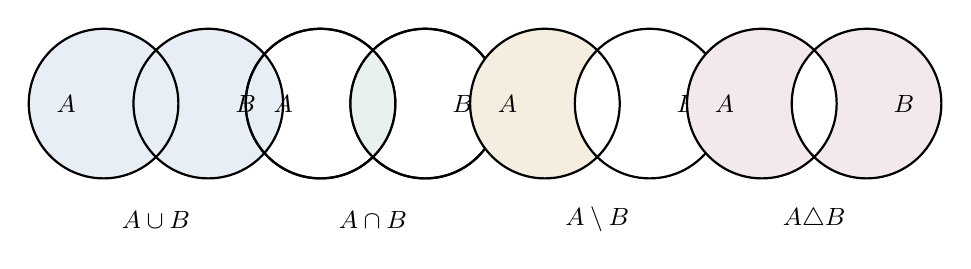
\begin{tikzpicture}[scale=0.95]
    % Three labelled regions: union (left), intersection (middle), difference + symdiff (right).

    % --- Union (everything shaded) ---
    \begin{scope}[shift={(-4.4,0)}]
        \fill[ideaBack] (-0.7,0) circle (1.0);
        \fill[ideaBack] ( 0.7,0) circle (1.0);
        \draw[thick] (-0.7,0) circle (1.0);
        \draw[thick] ( 0.7,0) circle (1.0);
        \node at (-1.2, 0.0) {\small $A$};
        \node at ( 1.2, 0.0) {\small $B$};
        \node at (0,-1.55) {\small $A \cup B$};
    \end{scope}

    % --- Intersection (only the lens shaded) ---
    \begin{scope}[shift={(-1.5,0)}]
        \draw[thick] (-0.7,0) circle (1.0);
        \draw[thick] ( 0.7,0) circle (1.0);
        \begin{scope}
            \clip (-0.7,0) circle (1.0);
            \fill[exBack] (0.7,0) circle (1.0);
        \end{scope}
        \draw[thick] (-0.7,0) circle (1.0);
        \draw[thick] ( 0.7,0) circle (1.0);
        \node at (-1.2, 0.0) {\small $A$};
        \node at ( 1.2, 0.0) {\small $B$};
        \node at (0,-1.55) {\small $A \cap B$};
    \end{scope}

    % --- Difference A \ B (left lune only shaded) ---
    \begin{scope}[shift={(1.5,0)}]
        \begin{scope}
            \clip (-0.7,0) circle (1.0);
            \fill[warnBack] (-2,-2) rectangle (2,2);
            \fill[white]    ( 0.7,0) circle (1.0);
        \end{scope}
        \draw[thick] (-0.7,0) circle (1.0);
        \draw[thick] ( 0.7,0) circle (1.0);
        \node at (-1.2, 0.0) {\small $A$};
        \node at ( 1.2, 0.0) {\small $B$};
        \node at (0,-1.55) {\small $A \setminus B$};
    \end{scope}

    % --- Symmetric difference (both lunes shaded, lens unshaded) ---
    \begin{scope}[shift={(4.4,0)}]
        \begin{scope}
            \clip (-0.7,0) circle (1.0);
            \fill[noteBack] (-2,-2) rectangle (2,2);
            \fill[white]    ( 0.7,0) circle (1.0);
        \end{scope}
        \begin{scope}
            \clip ( 0.7,0) circle (1.0);
            \fill[noteBack] (-2,-2) rectangle (2,2);
            \fill[white]    (-0.7,0) circle (1.0);
        \end{scope}
        \draw[thick] (-0.7,0) circle (1.0);
        \draw[thick] ( 0.7,0) circle (1.0);
        \node at (-1.2, 0.0) {\small $A$};
        \node at ( 1.2, 0.0) {\small $B$};
        \node at (0,-1.55) {\small $A \triangle B$};
    \end{scope}
\end{tikzpicture}
\end{center}

The fifth operation, \emph{subset testing} ($A \subseteq B$), is not
a Venn region --- it is a yes/no predicate (``is $A$'s circle
entirely inside $B$'s circle?''). Subsection below.

\subsection*{C++ implementations}

The \texttt{<algorithm>} header provides set operations on \emph{sorted ranges}, which means any sorted container:

\begin{lstlisting}[basicstyle=\ttfamily\small,frame=single]
#include <set>
#include <algorithm>
#include <iterator>

std::set<int> a{54, 19, 75}, b{75, 12}, out;

std::set_union(a.begin(), a.end(), b.begin(), b.end(),
               std::inserter(out, out.end()));
// out = {12, 19, 54, 75}

out.clear();
std::set_intersection(a.begin(), a.end(), b.begin(), b.end(),
                      std::inserter(out, out.end()));
// out = {75}

out.clear();
std::set_difference(a.begin(), a.end(), b.begin(), b.end(),
                    std::inserter(out, out.end()));
// out = {19, 54}
\end{lstlisting}

For \texttt{std::unordered\_set}, you write the loops explicitly:

\begin{lstlisting}[basicstyle=\ttfamily\small,frame=single]
std::unordered_set<int> setUnion(const std::unordered_set<int>& a,
                                 const std::unordered_set<int>& b) {
    std::unordered_set<int> r(a);
    r.insert(b.begin(), b.end());
    return r;
}

std::unordered_set<int> setIntersect(const std::unordered_set<int>& a,
                                     const std::unordered_set<int>& b) {
    // Iterate the smaller one -- saves time.
    const auto& smaller = a.size() <= b.size() ? a : b;
    const auto& larger  = a.size() <= b.size() ? b : a;
    std::unordered_set<int> r;
    for (int x : smaller)
        if (larger.count(x)) r.insert(x);
    return r;
}

std::unordered_set<int> setDiff(const std::unordered_set<int>& a,
                                const std::unordered_set<int>& b) {
    std::unordered_set<int> r;
    for (int x : a)
        if (!b.count(x)) r.insert(x);
    return r;
}
\end{lstlisting}

\begin{warnbox}
\textbf{Always iterate the smaller set.} For intersection, this shaves the cost from $O(|A|)$ to $O(\min(|A|, |B|))$ -- a huge win when one side is tiny. It's the single most common optimization in real set-heavy code.
\end{warnbox}

\subsection*{Cost analysis}

Assume hash-based sets with $O(1)$ expected insert and lookup.

\begin{center}
\begin{tabular}{lll}
\hline
Operation & Cost & Why \\
\hline
Union $|A| + |B|$ & $O(|A| + |B|)$ & insert all \\
Intersection & $O(\min(|A|, |B|))$ & scan smaller, probe larger \\
Difference $A \setminus B$ & $O(|A|)$ & scan $A$, probe $B$ \\
Subset $A \subseteq B$ & $O(|A|)$ & scan $A$, probe $B$ \\
\hline
\end{tabular}
\end{center}

For sorted (tree) sets, add a $\log n$ factor for each membership probe.

\begin{ideabox}
\textbf{Sorted vs.\ hashed, revisited.} With sorted sets, the two-pointer merge algorithm computes union/intersection/difference in $O(|A| + |B|)$, matching the hashed version without any per-element hash. On small sets that fit in cache, the sorted version can actually be \emph{faster}, because hashing has nontrivial constant overhead. For large sets with large element types, hashed wins. Benchmark before picking.
\end{ideabox}

\begin{defnbox}
\textbf{Algorithmic difference: sorted-merge vs.\ hash-probe.} The
two impl families compute the same set-theoretic answer via
fundamentally different algorithms:

\begin{itemize}[leftmargin=*]
    \item \textbf{Sorted-merge} (any sorted-range impl ---
          \texttt{std::set}, \texttt{std::vector} after \texttt{sort},
          B-tree leaf scan): two pointers walk $A$ and $B$ in
          lock-step. Each comparison advances at least one pointer.
          Total work: $\Theta(|A| + |B|)$
          \emph{deterministic worst case}, no hashing required.
    \item \textbf{Hash-probe} (\texttt{std::unordered\_set} +
          \texttt{count} loop): for each element of one set, a
          single hash + bucket-probe against the other.
          $O(|A| + |B|)$ \emph{expected} (assuming a well-distributed
          hash), but $O(|A| \cdot |B|)$ worst case under adversarial
          hash collisions.
\end{itemize}

The two are asymptotically equivalent in the average case. They
diverge on (a) constants (hashing eats $\sim 50$--$200$ cycles per
op even when the bucket lookup is $O(1)$; merge does pure
comparisons, no hash), (b) cache locality (sorted-merge streams two
arrays linearly; hash-probe touches random bucket addresses), and
(c) worst-case guarantees (sorted-merge is deterministic; hash is
amortised + assumes good hash).
\end{defnbox}

\begin{examplebox}[Sorted-merge vs.\ hash-probe, worked]
$A = \{1, 3, 5, 7\}$, $B = \{3, 4, 5, 6\}$.

\textbf{Sorted-merge $A \cup B$ on \texttt{std::set}:}
\begin{itemize}[leftmargin=*]
    \item Initialise pointers $i, j = 0, 0$. Output $\{\}$.
    \item Compare $A[0]=1, B[0]=3$: $1 < 3$, emit $1$, $i \to 1$.
          Output $\{1\}$.
    \item Compare $A[1]=3, B[0]=3$: equal, emit $3$, advance both.
          Output $\{1, 3\}$.
    \item Compare $A[2]=5, B[1]=4$: $5 > 4$, emit $4$, $j \to 2$.
          Output $\{1, 3, 4\}$.
    \item Compare $A[2]=5, B[2]=5$: equal, emit $5$, advance both.
          Output $\{1, 3, 4, 5\}$.
    \item Compare $A[3]=7, B[3]=6$: $7 > 6$, emit $6$, $j \to 4$
          (exhausted). Output $\{1, 3, 4, 5, 6\}$.
    \item Drain $A$: emit $7$. Output $\{1, 3, 4, 5, 6, 7\}$.
    \item \emph{Cost}: 5 comparisons + 6 emits.
          $\Theta(|A| + |B|) = \Theta(8)$ work; zero hashes.
\end{itemize}

\textbf{Hash-probe $A \cup B$ on \texttt{std::unordered\_set}:}
\begin{itemize}[leftmargin=*]
    \item Copy $A$ into output: 4 hashes + 4 inserts. Output
          $\{1, 3, 5, 7\}$.
    \item For each $b \in B$: hash $b$, probe output, insert if
          absent.
          \begin{itemize}
              \item $b=3$: hash, probe finds it, no insert.
              \item $b=4$: hash, probe miss, insert.
              \item $b=5$: hash, probe finds it, no insert.
              \item $b=6$: hash, probe miss, insert.
          \end{itemize}
          Output $\{1, 3, 4, 5, 6, 7\}$ (\emph{unordered}).
    \item \emph{Cost}: 8 hashes + 6 bucket probes + 6 inserts.
          $O(|A| + |B|)$ expected; constant factor $\sim 3 \times$
          higher than sorted-merge for small int keys due to hash
          cost.
\end{itemize}

Both produce the same set; sorted-merge produces \emph{sorted output
for free}, hash-probe gives no order guarantee.
\end{examplebox}

\subsection*{Symmetric difference}

\begin{defnbox}
\textbf{Symmetric difference.} $A \triangle B$ is the set of
elements in \emph{exactly one} of $A$ and $B$:
\[
A \triangle B \;=\; (A \setminus B) \cup (B \setminus A)
\;=\; (A \cup B) \setminus (A \cap B).
\]
Commutative ($A \triangle B = B \triangle A$); not associative
beyond the standard set-theoretic identity.
\end{defnbox}

The \texttt{<algorithm>} header provides this directly on sorted
ranges:

\begin{lstlisting}[basicstyle=\ttfamily\small,frame=single]
#include <set>
#include <algorithm>
#include <iterator>

std::set<int> a{1, 3, 5, 7}, b{3, 4, 5, 6}, out;
std::set_symmetric_difference(
    a.begin(), a.end(), b.begin(), b.end(),
    std::inserter(out, out.end()));
// out = {1, 4, 6, 7}
\end{lstlisting}

For unordered sets, the hand-rolled form is
\verb|setUnion(setDiff(a, b), setDiff(b, a))| or, equivalently,
$O(|A| + |B|)$ via two scan-and-probe passes. Use cases: change
detection between two snapshots ($A$ = ``yesterday's user IDs,'' $B$
= ``today's''; $A \triangle B$ = churn), file diffs, version-control
``these lines are in exactly one of the two revisions.''

\subsection*{Subset testing, formally}

The \texttt{isSubset} algorithm sketched in \S12.1 is the canonical
form. Cost analysis warrants a separate look:

\begin{itemize}[leftmargin=*]
    \item \textbf{Hashed superset:} $O(|A|)$ expected, since each
          $\texttt{contains}_B(a)$ is $O(1)$ expected.
    \item \textbf{Sorted (tree / B-tree) superset:}
          $O(|A| \cdot \log |B|)$ deterministic --- one tree probe
          per element of $A$.
    \item \textbf{Both sides sorted:} fall back to a sorted-merge
          variant. Two pointers, advance the smaller; if at any
          point you advance off the end of $A$ before exhausting it
          via matches, $A \not\subseteq B$. Cost $O(|A| + |B|)$ ---
          \emph{tighter than $|A| \log |B|$ when $|A|$ is close to
          $|B|$}, looser when $|A| \ll |B|$.
\end{itemize}

The pick: hashed superset for small $|A|$ relative to $|B|$
(``does this 5-element query set fit inside this million-element
cache?''); sorted-merge for $|A| \approx |B|$
(``are these two billion-row tables equal?'').

Strict subset ($A \subseteq B$ \emph{and} $A \ne B$) is the same
algorithm plus a $|A| < |B|$ check.

\subsection*{Power set}

\begin{defnbox}
\textbf{Power set.} $\mathcal{P}(X) = \{S : S \subseteq X\}$ --- the
set of all subsets of $X$, including $\emptyset$ and $X$ itself.
$|\mathcal{P}(X)| = 2^{|X|}$.
\end{defnbox}

Brute enumeration: each subset corresponds to a length-$n$ bitmask
where bit $i$ indicates whether $X[i]$ is included. C++:

\begin{lstlisting}[basicstyle=\ttfamily\small,frame=single]
#include <vector>
#include <cstdint>

template<typename T>
std::vector<std::vector<T>> powerSet(const std::vector<T>& xs) {
    const std::size_t n = xs.size();
    std::vector<std::vector<T>> result;
    result.reserve(1ULL << n);                // 2^n
    for (std::uint64_t mask = 0; mask < (1ULL << n); ++mask) {
        std::vector<T> sub;
        for (std::size_t i = 0; i < n; ++i)
            if (mask & (1ULL << i)) sub.push_back(xs[i]);
        result.push_back(std::move(sub));
    }
    return result;
}
\end{lstlisting}

Cost: $\Theta(n \cdot 2^n)$ time and space. Practical only for
$n \le 20$-ish ($2^{20} \approx 10^6$); past that, you do not
\emph{enumerate} the power set, you \emph{iterate} subsets lazily
(same loop, no materialised \texttt{result}).

\begin{notebox}
\textbf{Why this lives in the bitset corner of the chapter.}
The \texttt{mask} variable above is a single-word bitset over the
universe $\{0, 1, \ldots, n-1\}$. Power-set enumeration is the
canonical use case for the bitset representation in \S12.5: when
the universe is small enough to fit in a 64-bit word, every subset
\emph{is} a single \texttt{uint64\_t}. Set ops on the subsets
become bitwise ops on the words.
\end{notebox}

\subsection*{Filter and map}

Two higher-order operations borrowed from functional programming:

\begin{defnbox}
\textbf{Filter.} Given a predicate $p$, return the subset of elements for which $p$ is true.

\textbf{Map.} Given a function $f$, return the set $\{f(x) : x \in X\}$. The result may be smaller than the input if $f$ is not injective (multiple inputs can map to the same output).
\end{defnbox}

\begin{lstlisting}[basicstyle=\ttfamily\small,frame=single]
#include <unordered_set>
#include <functional>

template<typename T, typename Pred>
std::unordered_set<T> setFilter(const std::unordered_set<T>& s, Pred p) {
    std::unordered_set<T> r;
    for (const auto& x : s) if (p(x)) r.insert(x);
    return r;
}

template<typename T, typename U, typename Fn>
std::unordered_set<U> setMap(const std::unordered_set<T>& s, Fn f) {
    std::unordered_set<U> r;
    for (const auto& x : s) r.insert(f(x));
    return r;
}

// Usage:
auto evens = setFilter(nums, [](int x){ return x % 2 == 0; });
auto lengths = setMap<std::string, size_t>(words,
                   [](const std::string& w){ return w.size(); });
\end{lstlisting}

Python / JavaScript / Rust / Haskell / Scala all have these as first-class methods on their set (and collection) types. C++ got closer in C++20 with \texttt{std::ranges::filter\_view} and \texttt{std::ranges::transform\_view}, but the syntax is still clunky compared to \texttt{xs.filter(...).map(...)} in better-styled languages.

\begin{notebox}
\textbf{Filter is a subset; map is not always.} Filter always returns a subset of the original. Map can shrink the set if collisions occur under $f$: $\{1, -1\} \to \{1\}$ via $f(x) = x^2$. If you need one-to-one semantics, use a list or multiset and track duplicates explicitly.
\end{notebox}

\section{12.3 Static vs.\ Dynamic Sets}

\begin{defnbox}
\textbf{Dynamic set.} Can be modified after construction -- supports add and remove.
\textbf{Static set.} Fixed at construction time. Supports read-only and new-set-producing operations (union, intersection, filter, \ldots), but not in-place add or remove.
\end{defnbox}

\begin{center}
\begin{tabular}{lll}
\hline
Operation & Dynamic & Static \\
\hline
Construct from collection & yes & yes \\
Count elements & yes & yes \\
Search / contains & yes & yes \\
\textbf{Add} & yes & no \\
\textbf{Remove} & yes & no \\
Union / intersection / difference (return new) & yes & yes \\
Filter / map (return new) & yes & yes \\
\hline
\end{tabular}
\end{center}

\subsection*{Why would you ever want a static set?}

\begin{ideabox}
A static set is \emph{immutable}. That buys you several things a mutable set can't:
\begin{itemize}[leftmargin=*]
    \item \textbf{Thread safety for free.} If nothing can change, no locks are needed.
    \item \textbf{Aggressive optimization.} The implementation can use a perfect hash (no collisions), a sorted array (cache-friendly, no per-bucket pointers), or compile-time constants.
    \item \textbf{Safe sharing.} Hand the same set to a dozen consumers and no one can break it.
    \item \textbf{Hashability.} An immutable set can itself be a key in another set or map. (Python's \texttt{frozenset} exists for exactly this.)
\end{itemize}
\end{ideabox}

\subsection*{Choosing in practice}

\begin{center}
\begin{tabular}{ll}
\hline
Use case & Choice \\
\hline
Allowed-country codes loaded at startup & Static -- set once, read forever \\
Stop-words for a search engine & Static -- fixed per language \\
Users currently online & Dynamic -- changes constantly \\
Session IDs issued today & Dynamic -- grows over time \\
Finalized vote tallies (after the election) & Static -- sealed after a deadline \\
Shopping cart contents & Dynamic -- user modifies it \\
\hline
\end{tabular}
\end{center}

\subsection*{C++ idioms for static sets}

C++ doesn't have a built-in frozen set. Common workarounds:

\begin{lstlisting}[basicstyle=\ttfamily\small,frame=single]
// 1. Wrap in const.
const std::unordered_set<std::string> STOP_WORDS{"a", "an", "the", "of"};

// 2. C++17 initializer at static scope.
constexpr std::array<int, 4> ALLOWED_CODES{200, 301, 302, 404};
// Binary-search in a sorted array -- cache-friendly, no dynamic allocation.

// 3. Compile-time perfect hash via gperf, for pathological performance.
\end{lstlisting}

\subsection*{Perfect hashing for static sets}

\begin{defnbox}
\textbf{Perfect hash function.} A hash function $h : U \to
\{0, \ldots, m-1\}$ that is \emph{injective on a fixed key set $S
\subseteq U$}: distinct $x, y \in S$ map to distinct slots. No
collisions, ever, for any $x \in S$. This gives $O(1)$
\emph{worst-case} (not just expected) lookup.
\end{defnbox}

Perfect hashing requires the key set to be known up front (\emph{the
set must be static}); given that, you can construct a hash function
custom-tailored to those keys.

The canonical construction is \textbf{FKS} (Fredman, Komlós, and
Szemerédi, 1984) --- a two-level scheme. CLRS \S11.5 walks the
proof; the architecture in two sentences:

\begin{enumerate}[leftmargin=*]
    \item \textbf{Level 1.} Hash all $n$ keys into a primary table
          of size $m_1 = n$ slots using a universal hash $h_1$.
          Some slots will collide --- expected.
    \item \textbf{Level 2.} For each level-1 slot containing $k$
          keys, allocate a secondary hash table of size $m_2 = k^2$
          and pick a level-2 hash $h_2$ (drawn from the same
          universal family) such that all $k$ keys land in
          distinct level-2 slots. The $k^2$ size ensures a perfect
          $h_2$ exists with probability $\ge 1/2$ --- a few
          rejection-sampling rounds find one.
\end{enumerate}

Total expected space: $O(n)$ (the $\sum k_i^2$ telescopes to $O(n)$
under universal hashing). Lookup: two hash evaluations + two slot
reads. \textbf{Strictly $O(1)$ worst case for any key in $S$.}

In production: \texttt{gperf} (GNU Perfect Hash Function Generator)
takes a list of strings at build time and emits a C/C++ hash
function and lookup table. Used for keyword sets in compilers,
HTTP-header tables, MIME types, anywhere the universe is small,
fixed, and lookup speed matters. Modern alternatives include
\texttt{cmph} (C minimal perfect hashing library) and
\texttt{phf} (Rust's compile-time perfect-hash crate).

\textbf{When to reach for it:} static set, small enough that
construction time is not a barrier ($\le 10^5$ keys is comfortable;
$10^6$ is feasible), and the marginal cost of expected-case-only
lookup matters --- compiler keyword tables, kernel syscall tables,
embedded firmware look-up.

\begin{notebox}[Sealed / frozen sets in modern languages]
The ``the set will never change after construction'' contract is
expressed structurally in most languages other than C++:
\begin{itemize}[leftmargin=*]
    \item \textbf{Python:} \texttt{frozenset(\{1, 2, 3\})} is a
          first-class type; mutation methods (\texttt{add},
          \texttt{discard}) do not exist on it. Hashable ---
          a \texttt{frozenset} can be a key in another set or
          dict.
    \item \textbf{Java:} \texttt{Set.of(1, 2, 3)} (Java 9+)
          returns an immutable \texttt{Set<Integer>}; mutation
          throws \texttt{UnsupportedOperationException}.
          Older Java code uses
          \texttt{Collections.unmodifiableSet(...)}.
    \item \textbf{Rust:} idiom is \texttt{BTreeSet} or
          \texttt{HashSet} bound through an immutable reference
          (\texttt{\&BTreeSet<T>}); the borrow checker enforces
          no-mutation statically. The \texttt{phf} crate gives
          true compile-time perfect-hash sets with zero runtime
          construction cost.
    \item \textbf{Haskell / OCaml:} all collections are immutable
          by default; ``frozen'' is the only flavour.
\end{itemize}
The C++ workarounds in the listing above approximate this
structural guarantee through convention --- \texttt{const}-wrapping
and \texttt{constexpr std::array} are syntactic shields, not
structural ones. The next subsection's notebox elaborates.
\end{notebox}

\begin{notebox}
\textbf{Immutability is a spectrum.} ``Const'' in C++ is syntactic -- someone can still \texttt{const\_cast} it away. Python's \texttt{frozenset} is structurally immutable. Rust and Haskell make the distinction first-class. If your codebase has a convention that ``const means truly immutable,'' lean into static sets; if not, you're one \texttt{const\_cast} from heisenbugs.
\end{notebox}

\subsection*{Sets you'll actually use}

\begin{center}
\begin{tabular}{lll}
\hline
Container & Order & Typical implementation \\
\hline
\texttt{std::set} & sorted & red-black tree (ch.\ 9) \\
\texttt{std::unordered\_set} & hash order & open-addressed hash table \\
\texttt{std::multiset} & sorted, allows dups & red-black tree \\
Python \texttt{set} & hash order & open-addressed hash table \\
Python \texttt{frozenset} & hash order & immutable hash table \\
Java \texttt{HashSet} / \texttt{TreeSet} & -- & hash / red-black \\
Rust \texttt{HashSet} / \texttt{BTreeSet} & -- & hash / B-tree \\
\hline
\end{tabular}
\end{center}

\section{12.4 Multiset (duplicates allowed)}

\begin{defnbox}
\textbf{Multiset / bag.} A collection like a Set, but each element
carries a \emph{multiplicity} $m(x) \ge 0$ (a non-negative integer) ---
the number of copies. A standard set is the multiset where
$m(x) \in \{0, 1\}$ for all $x$. Order is still incidental; what
changes is that $\{1, 1, 3\}$ and $\{1, 3\}$ are different multisets
(different multiplicity for $1$).
\end{defnbox}

The terms ``multiset'' and ``bag'' are interchangeable in
algorithm-textbook usage; ``multiset'' is the C++ STL spelling
(\texttt{std::multiset} / \texttt{std::multimap}).

\subsection*{The STL multiset, three behavioural deltas}

\texttt{std::multiset<K>} is RB-backed (same as \texttt{std::set}),
ordered, allows duplicates. The three operations whose behaviour
\emph{changes} versus \texttt{std::set}:

\begin{itemize}[leftmargin=*]
    \item \textbf{\texttt{count(k)} returns 0 or more} (vs.\ 0 or 1
          on \texttt{std::set}). Cost
          $O(\log n + m(k))$ --- one tree probe to find the first
          occurrence, then a linear scan of the duplicates run.
    \item \textbf{\texttt{erase(k)} removes ALL occurrences} of $k$
          (vs.\ at most one on \texttt{std::set}). To remove a
          single occurrence, take an iterator from \texttt{find(k)}
          and \texttt{erase(it)}.
    \item \textbf{\texttt{equal\_range(k)} returns
          $[\texttt{lower\_bound}, \texttt{upper\_bound})$} ---
          the half-open range of all occurrences of $k$. The
          canonical way to iterate all duplicates without
          re-probing.
\end{itemize}

\begin{lstlisting}[basicstyle=\ttfamily\small,frame=single]
#include <set>
#include <iostream>

std::multiset<int> ms{1, 3, 3, 3, 5, 7};

std::cout << ms.count(3);             // 3
ms.erase(3);                          // removes ALL three 3s
// ms is now {1, 5, 7}

ms.insert({2, 2, 2, 4});
auto [lo, hi] = ms.equal_range(2);
for (auto it = lo; it != hi; ++it)
    std::cout << *it << ' ';          // 2 2 2

// Remove exactly one occurrence of 2.
ms.erase(ms.find(2));
\end{lstlisting}

\subsection*{Set ops on multisets, contrasted}

The set-theoretic operations generalise to multisets, but
\emph{multiplicities have to be combined}, and the choice of
combiner is the only thing the standard does not legislate.

\begin{center}
\begin{tabular}{lll}
\hline
Op & Set rule & Multiset rule (multiplicities) \\
\hline
$A \cup B$ &
$x \in A \lor x \in B$ &
$m_A(x) + m_B(x)$ \emph{(sum, default)} \\
$A \cup B$ (alt) &
--- &
$\max(m_A(x), m_B(x))$ \emph{(max, also valid)} \\
$A \cap B$ &
$x \in A \land x \in B$ &
$\min(m_A(x), m_B(x))$ \\
$A \setminus B$ &
$x \in A \land x \notin B$ &
$\max(0, m_A(x) - m_B(x))$ \\
$A \triangle B$ &
$(A \setminus B) \cup (B \setminus A)$ &
$|m_A(x) - m_B(x)|$ \\
$A \subseteq B$ &
$\forall x: x \in A \Rightarrow x \in B$ &
$\forall x: m_A(x) \le m_B(x)$ \\
\hline
\end{tabular}
\end{center}

\begin{notebox}[Multiset union: sum vs.\ max]
The literature does not pick: CLRS does not legislate, the C++
standard's \texttt{std::set\_union} on \texttt{std::multiset} ranges
implements neither in full --- it produces the
\emph{max-multiplicities} result (one copy per distinct duplicate
between the two ranges). \texttt{std::multiset::merge}, by contrast,
gives \emph{sum-multiplicities} (every element from both sources
ends up in the destination).

\textbf{This chapter's default: sum-multiplicities.} It matches
\texttt{merge}, matches the algebraic identity
$|A \cup B| = |A| + |B| - |A \cap B|$ (which only holds with sum
+ min on multisets), and is what production code in counting /
inventory / histogram contexts actually means by ``union.''
Document whichever convention you pick at the call site --- the
convention is the contract.
\end{notebox}

\subsection*{Cross-link: heaps as multisets}

\textbf{ch.~7 (heaps)} already works on multiset semantics: a
priority queue with two equal-priority elements stores both. The
heap-property comparison uses $\le$ (or $\ge$ for max-heaps), not
$<$ --- this is the multiset-friendly form, and it lets duplicate
priorities coexist in the heap without pseudo-tiebreaking. Almost
every concrete impl in cs-300 (heap, BST, hash table) extends to
multisets by relaxing one strict-inequality to non-strict. ch.~7's
gap-analysis Set/Multiset note made this explicit; \S12.4 is the
ADT-side framing.

\section{12.5 Bitset / characteristic vector}

\begin{defnbox}
\textbf{Bitset (characteristic vector).} A direct-access array
representation of a Set over a small dense universe
$U = \{0, 1, \ldots, n-1\}$: an $n$-bit array where bit $i$ is $1$
iff $i \in S$. Membership is a single bit read; insert / erase are
single bit writes. $O(1)$ point-query. $O(n)$ space (where $n$ is
the universe size, \emph{not} the set cardinality).
\end{defnbox}

\begin{notebox}[When a bitset is the right Set impl]
Bitsets dominate when the key universe is \emph{small and dense}:
\begin{itemize}[leftmargin=*]
    \item \textbf{ASCII characters:} 128 bits = 16 bytes. The
          ``set of allowed delimiters'' for a parser.
    \item \textbf{Vertex IDs in a graph with} $|V| = 1000$:
          1000 bits $= 125$ bytes per visited-set. ch.~10's BFS /
          DFS visited-set is often a bitset in production.
    \item \textbf{Days of the year a job ran:} 365 bits = 46 bytes.
    \item \textbf{Compiler flag set, syscall flag set, CPU
          feature flags:} dozens to hundreds of bits.
\end{itemize}
The flip side: when the universe is \emph{sparse}
(``set of 64-bit integer IDs, in use $\sim 1\%$ of the space''), a
naive bitset is $2^{64}$ bits = 2 exabytes of zeros. Use a hash set
or a roaring bitmap (compressed bitset) instead.
\end{notebox}

\subsection*{Implementations}

C++ gives three flavours, picked by whether $n$ is known at compile
time:

\begin{itemize}[leftmargin=*]
    \item \textbf{\texttt{std::bitset<N>}} --- $N$ a compile-time
          constant. All ops are \texttt{constexpr}-eligible; the
          compiler often unrolls the word-loop. Fixed size; cannot
          grow or shrink at runtime. Standard-library, no extra
          dependencies.
    \item \textbf{\texttt{std::vector<uint64\_t>}} --- the
          hand-rolled form. Size is $\lceil N / 64 \rceil$ words;
          you write the indexing
          (\texttt{word = bits[i / 64]}, \texttt{mask = 1ULL << (i \% 64)}).
          Use this when $N$ is runtime-determined and you need
          word-level access for the bit-twiddling kernels.
    \item \textbf{\texttt{boost::dynamic\_bitset}} --- the
          production-grade runtime-sized bitset. Same word-array
          internals, plus growth / shrink, popcount, find-first /
          find-next, and the standard set-op overloads.
\end{itemize}

\subsection*{Set ops as bitwise ops}

Once both sides are bitset-encoded, every binary set operation
becomes a single bitwise instruction per word. Across $\lceil N/w \rceil$
words (where $w = 64$ on most CPUs):

\begin{center}
\begin{tabular}{ll}
\hline
Set op & Bitwise form \\
\hline
$A \cup B$ & \texttt{a |= b} (per word) \\
$A \cap B$ & \texttt{a \&= b} \\
$A \setminus B$ & \texttt{a \&= \~{}b} \\
$A \triangle B$ & \texttt{a \^{}= b} \\
$|S|$ (cardinality) & \texttt{popcount} per word, sum \\
contains$(i)$ & \texttt{(a[i/64] >> (i\%64)) \& 1} \\
\hline
\end{tabular}
\end{center}

All $O(\lceil N / w \rceil)$ word ops --- linear in universe size,
\emph{not} in set cardinality, and usually 32--64$\times$ faster
than the equivalent hash-set or tree-set impl due to word-level
parallelism + cache streaming. Modern CPUs have a dedicated
\texttt{popcnt} instruction (1 cycle latency); compilers emit it
for \texttt{std::popcount} (C++20) and \texttt{\_\_builtin\_popcount}.

\subsection*{The picture: a 64-bit word as a bitset}

\begin{center}
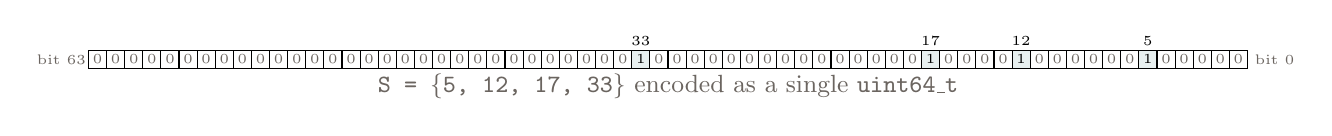
\begin{tikzpicture}[scale=0.23]
    % 64-bit word, drawn left = bit 63, right = bit 0 (standard CPU layout).
    \foreach \i in {0,...,63} {
        \pgfmathtruncatemacro{\bitidx}{63-\i}
        \pgfmathtruncatemacro{\highlight}{(\bitidx==5 || \bitidx==12 || \bitidx==17 || \bitidx==33) ? 1 : 0}
        \ifnum\highlight=1
            \fill[exBack] (\i,0) rectangle (\i+1,1);
            \draw (\i,0) rectangle (\i+1,1);
            \node[font=\tiny] at (\i+0.5, 0.5) {1};
        \else
            \draw (\i,0) rectangle (\i+1,1);
            \node[font=\tiny\color{mutedtext}] at (\i+0.5, 0.5) {0};
        \fi
    }
    % Position labels for the highlighted bits.
    \node[font=\tiny] at (63-5+0.5, 1.5) {5};
    \node[font=\tiny] at (63-12+0.5, 1.5) {12};
    \node[font=\tiny] at (63-17+0.5, 1.5) {17};
    \node[font=\tiny] at (63-33+0.5, 1.5) {33};
    \node[font=\small\color{mutedtext}] at (32, -1.0)
        {\texttt{S = \{5, 12, 17, 33\}} encoded as a single \texttt{uint64\_t}};
    \node[font=\tiny\color{mutedtext}] at (-1.5, 0.5) {bit 63};
    \node[font=\tiny\color{mutedtext}] at (65.5, 0.5) {bit 0};
\end{tikzpicture}
\end{center}

The diagram above shows the set $\{5, 12, 17, 33\}$ over the
universe $\{0, \ldots, 63\}$. Each set bit ($1$) is an element of
$S$; each clear bit ($0$) is absent. The whole set is one
\texttt{uint64\_t}: \texttt{S = (1ULL << 5) | (1ULL << 12) | (1ULL
<< 17) | (1ULL << 33)}.

\begin{examplebox}[Word-level bit-twiddling, worked]
Universe: $\{0, \ldots, 63\}$ (single 64-bit word).
$A = \{5, 12, 17\}$, $B = \{12, 17, 33\}$.

\begin{itemize}[leftmargin=*]
    \item Encode:
          \texttt{a = (1ULL<<5) | (1ULL<<12) | (1ULL<<17);}
          \texttt{b = (1ULL<<12) | (1ULL<<17) | (1ULL<<33);}
    \item \textbf{Set bit 5}: \texttt{a |= (1ULL << 5);}
          (idempotent --- already set; the \texttt{|=} is the
          right primitive even when you don't know whether the
          bit was already present).
    \item \textbf{Query bit 12}:
          \texttt{(a >> 12) \& 1ULL} returns $1$
          $\Rightarrow$ $12 \in A$.
    \item \textbf{Cardinality}:
          \texttt{std::popcount(a)} returns $3$;
          \texttt{std::popcount(b)} returns $3$.
    \item \textbf{Union} $A \cup B$:
          \texttt{u = a | b;}
          $\Rightarrow$ \texttt{popcount(u) == 4},
          set is $\{5, 12, 17, 33\}$.
    \item \textbf{Intersection} $A \cap B$:
          \texttt{i = a \& b;} $\Rightarrow$
          \texttt{popcount(i) == 2}, set is $\{12, 17\}$.
    \item \textbf{Difference} $A \setminus B$:
          \texttt{d = a \& \~{}b;} $\Rightarrow$
          \texttt{popcount(d) == 1}, set is $\{5\}$.
    \item \textbf{Symmetric difference} $A \triangle B$:
          \texttt{x = a \^{} b;} $\Rightarrow$
          \texttt{popcount(x) == 2}, set is $\{5, 33\}$.
    \item \textbf{Iterate the elements of $A$}: while
          \texttt{a != 0}, emit \texttt{std::countr\_zero(a)}
          (lowest set bit), then \texttt{a \&= a - 1} (clear it).
          Three iterations: emit 5, 12, 17.
\end{itemize}

Eight set-theoretic queries, each compiled to one or two CPU
instructions. The same operations on \texttt{std::unordered\_set}
would cost $\sim 100\times$ more cycles per op.
\end{examplebox}

\begin{notebox}[Forward direction: roaring bitmaps]
The bitset representation breaks down when the universe is
\emph{sparse} --- a 32-bit-int set with only $\sim 1000$ elements
would be $2^{32}$ bits $= 512$ MB of mostly zeros. Production
systems instead use \emph{roaring bitmaps}: a 32-bit ID is split
into a 16-bit ``container index'' + a 16-bit offset, and each
container is encoded as one of three shapes (sorted-array for
$\le 4096$ elements, dense bitset for $\ge 4096$, run-length
encoding for clustered runs). Set ops dispatch on the shape pair
and stay $O(\sqrt{n})$ per op on typical data. Used in
PostgreSQL's \texttt{bitmap} index scans, Apache Druid, Apache
Lucene, and ClickHouse. \texttt{CRoaring} (C / C++) is the
canonical implementation.
\end{notebox}

\section{12.6 Disjoint-Set Union (Union-Find)}

\begin{defnbox}
\textbf{Disjoint-Set Union (DSU), aka Union-Find.} A partition of
$n$ elements into $k$ pairwise disjoint sets. Three operations:
\begin{itemize}[leftmargin=*]
    \item \texttt{makeSet(x)}: create a new singleton $\{x\}$.
    \item \texttt{find(x)}: return a canonical representative
          (``root'') of the set currently containing $x$.
          Two elements are in the same set iff
          \texttt{find(x) == find(y)}.
    \item \texttt{unite(x, y)}: replace the two sets containing
          $x$ and $y$ with their union.
\end{itemize}
The data structure as a whole is itself a Set ADT --- a
\emph{set of disjoint sets}.
\end{defnbox}

\subsection*{Use cases}

\begin{itemize}[leftmargin=*]
    \item \textbf{Connectivity tracking.} ``Are $u$ and $v$ in the
          same connected component?'' Each \texttt{addEdge(u, v)}
          is a \texttt{unite}; each query is a \texttt{find}
          comparison.
    \item \textbf{Kruskal's MST (ch.~10 \S10.12).} Already covered
          in the chapter on graphs --- cycles in the partial MST
          are detected by ``the next edge $(u, v)$ has
          \texttt{find(u) == find(v)}.'' DSU is the
          algorithm-shaped reason Kruskal is $O(E \log E)$ and not
          $O(E \cdot V)$. Cross-link: ch.~10 \S10.12 has the
          Kruskal application; this section has the ADT framing.
    \item \textbf{Tarjan's offline strongly-connected-components.}
          Off-line variant of SCC computation that uses DSU
          instead of the recursion stack from ch.~10 \S10.6.
    \item \textbf{Online dynamic graph connectivity (incremental
          only).} DSU answers ``are $u$ and $v$ connected?'' under
          a stream of edge insertions in $O(\alpha(n))$ amortised
          per op. Decremental connectivity (edge \emph{removals})
          is much harder and needs different machinery.
    \item \textbf{Equivalence-class management.} Type-inference
          unification, image-segmentation flood fill, percolation
          theory.
\end{itemize}

\subsection*{Implementation: parent-pointer forest}

Each set is an \emph{up-tree}: every element points at a parent;
the root points at itself and is the canonical representative.
\texttt{find(x)} walks parent pointers to the root.
\texttt{unite(x, y)} computes \texttt{rx = find(x)} and
\texttt{ry = find(y)}, then makes one root the parent of the other.

\begin{lstlisting}[basicstyle=\ttfamily\small,frame=single]
struct DSU {
    std::vector<int> parent, rank_;
    explicit DSU(int n) : parent(n), rank_(n, 0) {
        for (int i = 0; i < n; ++i) parent[i] = i;
    }
    int find(int x) {
        // Path compression: every node on the find-path
        // points directly at the root after the call.
        return parent[x] == x ? x
                              : parent[x] = find(parent[x]);
    }
    bool unite(int x, int y) {
        int rx = find(x), ry = find(y);
        if (rx == ry) return false;            // already united
        // Union by rank: shorter tree under taller.
        if (rank_[rx] < rank_[ry]) std::swap(rx, ry);
        parent[ry] = rx;
        if (rank_[rx] == rank_[ry]) ++rank_[rx];
        return true;
    }
};
\end{lstlisting}

\subsection*{The two optimisations}

\begin{itemize}[leftmargin=*]
    \item \textbf{Union by rank (or size).} Each root carries a
          ``rank'' (an upper bound on tree height; in the
          size-based variant, the subtree's element count
          instead). When uniting two trees, the shorter one is
          attached under the taller. Without compression this
          alone gives $O(\log n)$ per op (depth $\le \log_2 n$).
    \item \textbf{Path compression.} During \texttt{find}, after
          locating the root, re-point every node on the find-path
          directly at the root. Flattens the tree
          \emph{lazily} --- the work is paid by the same query
          that needed the answer.
\end{itemize}

Either optimisation alone is $O(\log n)$. \emph{Together}, the
amortised cost per op drops to $O(\alpha(n))$, where $\alpha$ is
the inverse Ackermann function --- a function so slowly growing
that $\alpha(n) \le 4$ for any $n \le 2^{2^{2^{2^{16}}}}$
(approximately $2^{65536}$). For any input that fits in the
universe, DSU is effectively constant per operation.

\textbf{Theorem (Tarjan 1975, refined Tarjan--van Leeuwen 1984).}
The amortised cost of $m$ \texttt{find} / \texttt{unite}
operations on $n$ elements with both optimisations is
$\Theta(m \cdot \alpha(m, n))$. The matching lower bound shows
this is optimal in the pointer-machine model. CLRS Ch~21 walks
the proof; this chapter takes it as a black box.

\subsection*{The picture: parent forest, union step, path compression}

\begin{center}
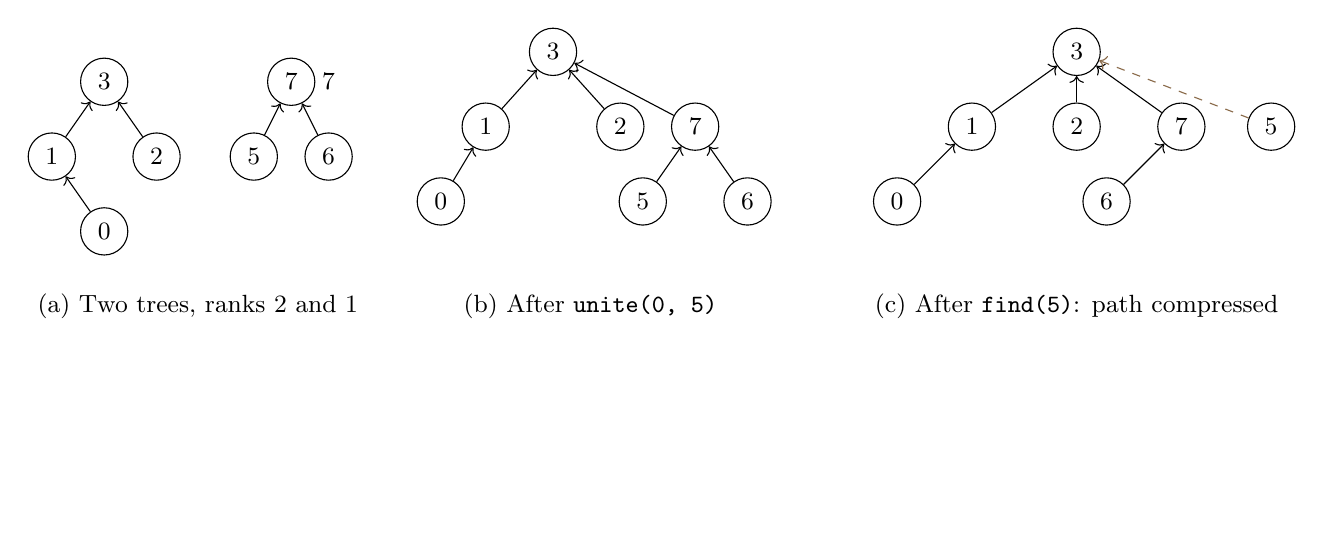
\begin{tikzpicture}[scale=0.95,
    every node/.style={circle, draw, minimum size=6mm,
                       inner sep=0pt, font=\small}]

    % --- (a) Two separate up-trees, before union.
    \begin{scope}[shift={(-5.0,0)}]
        \node (a3) at (0, 1.6) {3};
        \node (a1) at (-0.7, 0.6) {1};
        \node (a2) at (0.7, 0.6) {2};
        \node (a0) at (0, -0.4) {0};
        \draw[->] (a1) -- (a3);
        \draw[->] (a2) -- (a3);
        \draw[->] (a0) -- (a1);

        \node[draw=none] at (3.0, 1.6) {7};
        \node[draw=none] at (3.0, 0.6) {};
        \node (b7) at (2.5, 1.6) {7};
        \node (b5) at (2.0, 0.6) {5};
        \node (b6) at (3.0, 0.6) {6};
        \draw[->] (b5) -- (b7);
        \draw[->] (b6) -- (b7);

        \node[draw=none, font=\small] at (1.25, -1.4) {(a) Two trees, ranks $2$ and $1$};
    \end{scope}

    % --- (b) After unite(0, 5): rank-2 tree absorbs rank-1.
    \begin{scope}[shift={(0.5,0)}]
        \node (c3) at (0.5, 2.0) {3};
        \node (c1) at (-0.4, 1.0) {1};
        \node (c2) at (1.4, 1.0) {2};
        \node (c0) at (-1.0, 0.0) {0};
        \node (c7) at (2.4, 1.0) {7};
        \node (c5) at (1.7, 0.0) {5};
        \node (c6) at (3.1, 0.0) {6};
        \draw[->] (c1) -- (c3);
        \draw[->] (c2) -- (c3);
        \draw[->] (c0) -- (c1);
        \draw[->] (c7) -- (c3);
        \draw[->] (c5) -- (c7);
        \draw[->] (c6) -- (c7);

        \node[draw=none, font=\small] at (1.0, -1.4) {(b) After \texttt{unite(0, 5)}};
    \end{scope}

    % --- (c) After find(5): path compression.
    \begin{scope}[shift={(7.0,0)}]
        \node (d3) at (1.0, 2.0) {3};
        \node (d1) at (-0.4, 1.0) {1};
        \node (d2) at (1.0, 1.0) {2};
        \node (d0) at (-1.4, 0.0) {0};
        \node (d7) at (2.4, 1.0) {7};
        \node (d5) at (3.6, 1.0) {5};
        \node (d6) at (1.4, 0.0) {6};
        \draw[->] (d1) -- (d3);
        \draw[->] (d2) -- (d3);
        \draw[->] (d0) -- (d1);
        \draw[->] (d7) -- (d3);
        \draw[->, dashed, accent] (d5) -- (d3);
        \draw[->] (d6) -- (d7);

        \node[draw=none, font=\small] at (1.0, -1.4) {(c) After \texttt{find(5)}: path compressed};
    \end{scope}
\end{tikzpicture}
\end{center}

In panel (c), the dashed arrow shows the new direct parent edge
\texttt{5 -> 3} that path compression installed: previously $5 \to
7 \to 3$ (depth 2), now $5 \to 3$ (depth 1). Every subsequent
\texttt{find(5)} costs one parent read instead of two.

\begin{examplebox}[8-element DSU sequence, with path compression]
Universe $\{0, 1, \ldots, 7\}$, all initially singletons. Trace
the parent-pointer state through six ops:

\begin{enumerate}[leftmargin=*]
    \item Initial: \texttt{parent = [0,1,2,3,4,5,6,7]},
          \texttt{rank = [0,0,0,0,0,0,0,0]}.
    \item \texttt{unite(0, 1)}: $\text{find}(0)=0$,
          $\text{find}(1)=1$; ranks tied, attach $1 \to 0$ and
          bump \texttt{rank[0]=1}.
          \texttt{parent = [0,0,2,3,4,5,6,7]}.
    \item \texttt{unite(2, 3)}: same shape, attach $3 \to 2$,
          \texttt{rank[2]=1}.
          \texttt{parent = [0,0,2,2,4,5,6,7]}.
    \item \texttt{unite(0, 2)}: $\text{find}(0)=0$,
          $\text{find}(2)=2$; both rank-$1$, attach $2 \to 0$ and
          \texttt{rank[0]=2}.
          \texttt{parent = [0,0,0,2,4,5,6,7]}.
    \item \texttt{unite(4, 5)}: \texttt{parent = [0,0,0,2,4,4,6,7]},
          \texttt{rank[4]=1}.
    \item \texttt{unite(6, 7)}: \texttt{parent = [0,0,0,2,4,4,6,6]},
          \texttt{rank[6]=1}.
    \item \texttt{unite(4, 6)}: both rank-$1$, attach $6 \to 4$,
          \texttt{rank[4]=2}.
          \texttt{parent = [0,0,0,2,4,4,4,6]}.
    \item \texttt{unite(0, 7)}: $\text{find}(0)=0$ (one hop);
          $\text{find}(7)$: $7 \to 6 \to 4$, returns $4$.
          \emph{Path compression rewrites
          \texttt{parent[7]=4}.}
          Both ranks are 2, attach $4 \to 0$, \texttt{rank[0]=3}.
          \texttt{parent = [0,0,0,2,0,4,4,4]}.
\end{enumerate}

After step 8, \emph{everything} is in one set rooted at $0$. The
\texttt{find} on $7$ flattened the tree on the way through ---
the next \texttt{find(7)} costs one hop instead of three.
\end{examplebox}

\section{12.7 Bloom filter}

\begin{defnbox}
\textbf{Bloom filter.} A space-efficient probabilistic Set
membership data structure with \emph{one-sided error}:
\begin{itemize}[leftmargin=*]
    \item \texttt{contains(x) == false}: $x$ is \emph{definitely
          not} in the set. No false negatives, ever.
    \item \texttt{contains(x) == true}: $x$ is \emph{probably}
          in the set. False positives are possible at a tunable
          rate.
\end{itemize}
The structure is a single $m$-bit array plus $k$ independent hash
functions $h_1, \ldots, h_k : U \to \{0, \ldots, m-1\}$. Insert
$x$ by setting bits $h_1(x), \ldots, h_k(x)$; query by checking
that all $k$ bits are $1$.
\end{defnbox}

\subsection*{Construction and queries}

\begin{lstlisting}[basicstyle=\ttfamily\small,frame=single]
#include <vector>
#include <cstdint>
#include <functional>

class BloomFilter {
    std::vector<std::uint64_t> bits;     // m bits packed in 64-bit words
    std::size_t m;                        // bit count
    int k;                                // # hash functions

    std::size_t hash(std::size_t seed, std::uint64_t x) const {
        // Cheap two-hash trick: combine std::hash with a salt.
        return (std::hash<std::uint64_t>{}(x ^ seed)) % m;
    }
public:
    BloomFilter(std::size_t m_, int k_)
        : bits((m_ + 63) / 64, 0), m(m_), k(k_) {}

    void insert(std::uint64_t x) {
        for (int i = 0; i < k; ++i) {
            std::size_t b = hash(i * 0x9E3779B97F4A7C15ULL, x);
            bits[b / 64] |= (1ULL << (b % 64));
        }
    }
    bool contains(std::uint64_t x) const {
        for (int i = 0; i < k; ++i) {
            std::size_t b = hash(i * 0x9E3779B97F4A7C15ULL, x);
            if (!(bits[b / 64] & (1ULL << (b % 64)))) return false;
        }
        return true;            // probably present (or false positive)
    }
};
\end{lstlisting}

\textbf{No \texttt{erase}.} A naive Bloom filter cannot delete: any
bit set might be ``shared'' between multiple inserted keys, so
clearing it could turn a true positive into a false negative,
breaking the one-sided-error contract. The counting-Bloom variant
in the next notebox restores delete by replacing each bit with a
small counter.

\subsection*{The false-positive-rate formula}

After inserting $n$ keys into an $m$-bit table with $k$ hash
functions (assumed independent and uniform), the probability that
a specific bit is still $0$ is
$\left(1 - 1/m\right)^{kn} \approx e^{-kn/m}$.
A query for a never-inserted $y$ is a false positive iff all $k$ of
its bits happen to be set, which happens with probability:
\[
p \;\approx\; \bigl(1 - e^{-kn/m}\bigr)^k.
\]

Differentiating w.r.t.\ $k$ and setting $\frac{\partial p}{\partial k}=0$
gives the optimal number of hash functions:
\[
k^\star \;=\; \frac{m}{n} \ln 2 \;\approx\; 0.6931 \cdot \frac{m}{n}.
\]
At $k = k^\star$, the false-positive rate simplifies to
$p^\star = (1/2)^{k^\star}$, equivalently $m \approx -n \log_2 p^\star
/ \ln 2 \approx 1.44 \cdot n \cdot \log_2(1/p^\star)$ bits. Useful
calibrations:

\begin{center}
\begin{tabular}{rrr}
\hline
$p^\star$ & $m / n$ & $k^\star$ \\
\hline
0.10  & 4.79  & 4 \\
0.01  & 9.59  & 7 \\
0.001 & 14.38 & 10 \\
$10^{-4}$ & 19.18 & 14 \\
$10^{-5}$ & 23.97 & 17 \\
\hline
\end{tabular}
\end{center}

A 1\% false-positive rate costs $\sim 9.6$ bits per element.
Compare \texttt{std::unordered\_set}, which costs $\sim 32$ bytes
per element ($256\times$ more). That space ratio is the entire
business case for Bloom filters.

\subsection*{Use cases}

\begin{itemize}[leftmargin=*]
    \item \textbf{Database existence pre-check.} ``Is this key
          \emph{maybe} in the table?'' Avoid a disk read when the
          Bloom filter says no. RocksDB and LevelDB attach a
          per-SST-file Bloom filter so LSM compaction does not
          chase missing keys through every level.
    \item \textbf{CDN edge caching.} ``Is this URL \emph{maybe}
          in the cache?'' False-positive cost: one wasted RAM
          probe. False-negative cost: a cache miss that should
          have been a hit. The asymmetry justifies one-sided
          error.
    \item \textbf{Network packet filtering.} Squid web cache,
          firewall blacklist pre-checks. Cheap reject of known
          non-members before the expensive deep inspection.
    \item \textbf{DNS negative caching.} ``Have we recently failed
          to resolve this name?'' Bloom filter answers in
          microseconds; falling back on DNS itself takes
          milliseconds.
    \item \textbf{Distributed-systems set reconciliation.} Compare
          two large sets between nodes by exchanging Bloom
          filters first --- only fall back on full set
          reconciliation if the filters say there might be a
          difference.
\end{itemize}

\begin{notebox}[Variants beyond the textbook Bloom filter]
\begin{itemize}[leftmargin=*]
    \item \textbf{Counting Bloom filter.} Replace each bit with a
          $c$-bit counter (typically $c=4$). \texttt{insert}
          increments; \texttt{erase} decrements. False-positive
          analysis is unchanged but now you can \emph{remove}.
          $4\times$ space cost vs.\ a plain Bloom filter.
    \item \textbf{Cuckoo filter.} Stores small \emph{fingerprints}
          (8--16 bits) in a cuckoo-hash table; supports delete and
          gives a strictly better false-positive rate at the same
          space than counting Bloom. Used in CockroachDB.
    \item \textbf{Quotient filter / Xor filter.} Newer designs
          with cache-friendlier layouts; the Xor filter (Graf and
          Lemire, 2020) is read-only and matches Bloom space at
          $\sim 30\%$ better lookup throughput.
    \item \textbf{Scalable Bloom filter.} Chained Bloom filters
          that grow on demand --- maintains a target FPR even
          when $n$ is unknown a priori.
\end{itemize}
The original paper is Burton Bloom (1970); the canonical modern
survey is Broder and Mitzenmacher (\emph{Internet Mathematics},
2004), enumerated in \S12.8.
\end{notebox}

\section{12.8 Production references and further reading}

\begin{notebox}[Where Set impls actually live in production]
\textbf{C++ STL.}
\begin{itemize}[leftmargin=*]
    \item \texttt{std::set} / \texttt{std::map} ---
          red-black tree (cross-link \textbf{ch.~9}). Ordered
          iteration, \texttt{lower\_bound} / \texttt{upper\_bound},
          $O(\log n)$ worst case on all three core ops. The
          default ``ordered Set'' impl.
    \item \texttt{std::unordered\_set} /
          \texttt{std::unordered\_map} --- open-addressing or
          chained hash table (cross-link \textbf{ch.~5}).
          $O(1)$ expected on all three core ops; no order; the
          default ``unordered Set'' impl.
    \item \texttt{std::multiset} / \texttt{std::multimap} ---
          red-black tree with duplicate keys allowed. The three
          behavioural deltas in \S12.4 apply.
    \item \texttt{std::bitset<N>} --- compile-time-fixed bitset.
          \texttt{boost::dynamic\_bitset} is the runtime-sized
          counterpart.
\end{itemize}

\textbf{Higher-performance hash sets.}
\begin{itemize}[leftmargin=*]
    \item \texttt{absl::flat\_hash\_set} (Google Abseil) ---
          Swiss Tables open-addressing hash with SIMD-vectorised
          probing. $\sim 2$--$3 \times$ faster than
          \texttt{std::unordered\_set} on most workloads. Used
          inside Chrome, TensorFlow, Envoy.
    \item \texttt{phmap::flat\_hash\_set} (parallel-hashmap) ---
          drop-in replacement with sharded internal locking
          for concurrent use.
    \item \texttt{folly::F14ValueSet} (Facebook Folly) --- 14-way
          probe SIMD hash with a different layout / cache trade-off.
\end{itemize}

\textbf{Beyond C++.}
\begin{itemize}[leftmargin=*]
    \item Python \texttt{set} / \texttt{frozenset} --- open-
          addressing hash; \texttt{frozenset} is hashable.
    \item Java \texttt{HashSet} / \texttt{TreeSet} ---
          chained hash / red-black; Java 9+ \texttt{Set.of(...)}
          is the immutable form.
    \item Rust \texttt{HashSet} / \texttt{BTreeSet} --- hash
          (SipHash by default for HashDoS resistance) /
          B-tree-of-arrays (cross-link \textbf{ch.~11}).
\end{itemize}

\textbf{Specialised set structures.}
\begin{itemize}[leftmargin=*]
    \item \texttt{CRoaring} --- compressed bitmap library
          (cross-link \S12.5 forward-direction notebox). Used in
          Apache Druid, Lucene, ClickHouse, PostgreSQL bitmap
          scans.
    \item \texttt{libcuckoo} --- concurrent cuckoo hash set.
    \item RocksDB / LevelDB Bloom filter implementations --- one
          Bloom per SST file in the LSM tree.
\end{itemize}

\textbf{Canonical references.}
\begin{itemize}[leftmargin=*]
    \item \emph{CLRS} Ch~11 (hash tables), Ch~12 (BSTs as sets),
          Ch~13 (red-black trees), Ch~21 (disjoint-set
          structure).
    \item Broder and Mitzenmacher, \emph{``Network applications of
          Bloom filters: A survey,''} Internet Mathematics, 2004.
    \item Tarjan, \emph{``Efficiency of a good but not linear set
          union algorithm,''} JACM 22(2), 1975 --- the
          $\alpha(n)$ bound for DSU.
    \item Fredman, Komlós, Szemerédi, \emph{``Storing a sparse
          table with $O(1)$ worst case access time,''} JACM 31(3),
          1984 --- the FKS perfect-hash construction.
    \item Bloom, \emph{``Space/time trade-offs in hash coding with
          allowable errors,''} CACM 13(7), 1970 --- the original
          Bloom-filter paper.
    \item Mitzenmacher and Upfal, \emph{Probability and Computing}
          --- standard text for the probabilistic analyses
          underpinning Bloom filters and randomised data
          structures.
\end{itemize}
\end{notebox}

\begin{ideabox}
\textbf{Chapter takeaway.} Sets are the deduplicating, order-free,
membership-query-oriented sibling of lists. The chapter unifies
under the impl-decision matrix --- one ADT, seven impls, each tuned
to a different axis of the trade-off:
\begin{itemize}[leftmargin=*]
    \item \textbf{Hash set} (\textbf{ch.~5}, \texttt{std::unordered\_set}) --- $O(1)$ expected, no order.
          The default unless something else is needed.
    \item \textbf{Balanced BST} (\textbf{ch.~9},
          \texttt{std::set}) --- $O(\log n)$ worst case, ordered
          iteration, \texttt{lower\_bound}.
    \item \textbf{B-tree / B+ tree} (\textbf{ch.~11}, SQLite /
          PostgreSQL / MySQL InnoDB) --- $O(\log_K n)$, the
          on-disk version of the same operations.
    \item \textbf{Multiset} (\S12.4) --- duplicates allowed; one
          comparator relaxation.
    \item \textbf{Bitset} (\S12.5) --- small dense universe;
          $O(1)$ ops, $32$--$64\times$ faster constant than hash.
    \item \textbf{Disjoint-Set Union} (\S12.6) --- partition ADT;
          $O(\alpha(n))$ amortised; powers Kruskal (\textbf{ch.~10}
          \S10.12).
    \item \textbf{Bloom filter} (\S12.7) --- probabilistic, one-
          sided error; $\sim 10$ bits / element at $1\%$ FPR.
    \item \textbf{Perfect hash} (\S12.3) --- static set, $O(1)$
          \emph{worst} case; \texttt{gperf}, \texttt{phf}.
\end{itemize}
The recurring move: \emph{iterate one side, probe the other}, with
the probe shape (sorted-merge / hash-probe / bit-and) determined
by the impl pair. The ADT is simple; the engineering choices it
unlocks are not.

\textbf{Looking ahead.} Past the cs-300 boundary the Set ADT
extends in three directions. \emph{Concurrent / lock-free sets}:
Cliff Click's non-blocking hash map, Java's
\texttt{ConcurrentSkipListSet}, RCU-protected read-mostly sets,
and the lock-free hash-table research line (Michael 2002,
Shavit 2008). \emph{Sparse-bitmap research}: roaring bitmaps
(\S12.5 forward-direction notebox), tree-of-bitmaps, succinct
data structures with $H_0(n) + o(n)$ bits.
\emph{Set theory proper}: powerset lattices (the partial-order
structure on $\mathcal{P}(X)$), Boolean algebras, partial orders,
the connection from finite-set ADTs to the algebraic structures
that underpin databases (relational algebra is set algebra) and
type theory (subtyping is subset-of-values). cs-300 stops at the
ADT layer; the references in \S12.8 are the entry points for
continuing past it.
\end{ideabox}

\end{document}
